\chapter[Mutation]{Mutation testing}
\label{cap:preliminares.mutation}

\emph{Mutation testing} es un criterio de cobertura que puede ser considerado de \emph{caja blanca}, donde las metas a cubrir por la test suite est\'an representadas por fallas artificiales, que deben ser detectadas por la test suite bajo evaluaci\'on. Las fallas artificiales se representan a trav\'es de variantes del programa original, cada una de las cuales posee un cambio sint\'actico simple respecto al programa original, que representa un defecto. Cada variante se denomina \emph{mutante}, mientras que la falla artificial asociada se denomina \emph{mutaci\'on}. Cu\'antos de los mutantes generados son detectados por la test suite es el valor asociado a este criterio, y se denomina \emph{mutation score}.

Las fallas artificiales involucradas en mutation testing se producen en base a \emph{operadores de mutaci\'on}. Un operador de mutaci\'on define los cambios sint\'acticos que se van a realizar sobre un programa, t\'ipicamente eligiendo tipos particulares de expresiones en el mismo, y dando lugar a familias de mutantes. Dos ejemplos tradicionales de operadores de mutaci\'on son \emph{reemplazo de operadores relacionales}, el cual reemplaza un operador relacional por todos los otros soportados por el lenguaje de programaci\'on utilizado, y \emph{reemplazo de operadores aritm\'eticos}, que realiza cambios similares pero sobre operadores aritm\'eticos. La Figura~\ref{figures.examples.mutations} muestra un programa con varias mutaciones, en un mismo bloque de c\'odigo. Cada mutaci\'on est\'a indicada con $\Delta$, y sustituye la l\'inea (no mutada, es decir, sin $\Delta$) inmediata superior. Las mutaciones $1\Delta$, $2\Delta$ and $3\Delta$ en esta Figura corresponden a reemplazos de operadores relacionales, mientras que $4\Delta$ corresponde a reemplazo de operadores aritm\'eticos.

\begin{figure}[t]
	\begin{lstlisting}[frame=tlrb, mathescape=true,language=Java,basicstyle={},xleftmargin=.011\textwidth,xrightmargin=.011\textwidth]
   int countEven( int[] input ) {
     int count = 0;
     for (int i = 0; i < input.length; i++) {
     $1\Delta$for (int i = 0; i <= input.length; i++) {
     $2\Delta$for (int i = 0; i != input.length; i++) {
       int value = input[i];
       if (value % 2 == 0) {
       $3\Delta$ if (value % 2 != 0) {
         count = count + 1;
         $4\Delta$ count = count / 1;
       }
     }
     return count;
   }
	\end{lstlisting}
	\caption{Ejemplos de un programa y posibles mutaciones}
	\label{figures.examples.mutations}
\end{figure}

Al igual que en cualquier otro criterio de testing, mientras m\'as cercano al 100\% sea el valor asociado, m\'as confianza se puede tener en la calidad de la test suite evaluada. En el caso de mutation testing, este valor aumenta mientras m\'as mutantes sean detectados y disminuye en caso contrario. Sin embargo, existen situaciones que afectan de manera negativa a la confianza sobre este valor. Ciertas fallas son triviales de detectar, ya sea porque causan que la compilaci\'on o la ejecuci\'on (bajo cualquier entrada) falle, o s\'olo requieren alcanzabilidad para hacerlo. Por ejemplo, la sentencia

 \lstinline|if (c) x = array[-1];| 

\noindent
s\'olo requiere una entrada que satisfaga \emph{c} para detectar la falla. Ni siquiera es necesario un or\'aculo para evaluar el resultado: la ejecuci\'on genera una terminaci\'on abrupta, que manifiesta un bug. Las fallas triviales aumentan el mutation score sin implicar una mejora en la calidad de la test suite. En el espectro opuesto, puede haber fallas artificiales que tengan el mismo comportamiento sem\'antico que el c\'odigo original. Por ejemplo, la sentencia

 \lstinline|for (int i = 0; i < 10; i++)| 

\noindent
es equivalente a 

\lstinline|for (int i = 0; i < 10; ++i)|. 

\noindent
Estos mutantes son llamados equivalentes y por lo tanto indistinguibles del programa original, lo que genera metas que no pueden ser cubiertas, que a su vez disminuyen el valor de mutation score, aunque la test suite no tiene una peor calidad por no ser capaz de detectar estos mutantes. Finalmente, un valor alto de mutation score no significa nada si no existe una relaci\'on entre detectar fallas artificiales y reales. Discutiremos en mayor detalle esta \'ultima situaci\'on a continuaci\'on.

\pagebreak
\section{Operadores de mutaci\'on suficientes}
\label{sec:preliminares.mutation.sufficient}

El estudio llevado a cabo en \cite{bibliography.mutation.selection.Offutt96} evalu\'o el conjunto de operadores de mutaci\'on utilizados por \emph{Mothra}, una herramienta de mutation testing para el lenguaje Fortran-77. En este estudio, se define el siguiente conjunto de operadores, considerados \emph{suficientes}:

\begin{description}[leftmargin=8em,style=nextline]
	\item[ABS] Modifica cada expresi\'on aritm\'etica por 0, un valor positivo, y un valor negativo.
	\item[AOR] Reemplaza cada operador aritm\'etico por todos los operadores legales.
	\item[LCR] Reemplaza operadores l\'ogicos o condicionales por otros v\'alidos.
	\item[ROR] Reemplaza operadores relacionales.
	\item[UOI] Inserta operadores unarios en expresiones compatibles.
\end{description}

Intuitivamente, un conjunto de operadores se considera suficiente si la adici\'on de otros operadores de mutaci\'on no mejora la precisi\'on del mutation score como m\'etrica de la calidad de una suite. Si bien otros estudios sobre conjuntos suficientes de operadores se han realizado, entre ellos \cite{bibliography.mutation.selection.ASN2008}, todos arriban esencialmente a conclusiones similares. Por ejemplo, en \cite{bibliography.mutation.selection.ASN2008} se define un conjunto de operadores suficientes muy similar al previamente descripto, con la diferencia de que la herramienta de mutaci\'on utilizada en este \'ultimo ofrece una mayor cantidad de operadores de mutaci\'on, que en muchos casos est\'an inclu\'idos en los anteriores.

Cabe destacar que estos estudios siempre se ven afectados por la misma amenaza de validez: realizar el estudio bajo un conjunto de programas determinados con un conjunto de tests particulares no da necesariamente resultados generalizables a cualquier contexto de testing. Sin embargo, todos llegan al mismo conjunto de cambios, ya sea realizados por los mismos operadores o por operadores similares.

\pagebreak

\section{Propiedades de operadores de mutaci\'on}
\label{sec:preliminares.mutation.opevaluation}

En principio, un operador de mutaci\'on es una funci\'on que se aplica a elementos particulares de un programa, ya sea c\'odigo fuente o binarios, y genera versiones modificadas de \'estos. Desde el punto de vista de mutation testing, un operador de mutaci\'on a su vez debe tener un objetivo claro, como emular cierto tipo de fallas. Para que mutation testing sea un criterio efectivo, algunas propiedades deben ser tenidas en cuenta para el dise\~no de los operadores de mutaci\'on involucrados. La \emph{eficiencia temporal y relativa a otros recursos} obligan a que el conjunto de mutantes generados se mantenga acotado, de la misma forma en que, en el contexto general de testing, es necesario mantener al conjunto de tests a utilizar para evaluar un programa tambi\'en acotado. La \emph{efectividad} de mutation testing como forma de evaluar la calidad de una test suite, es decir, la habilidad de la suite para detectar potenciales fallas en un programa bajo an\'alisis, es otra caracter\'istica importante asociada a los operadores de mutaci\'on utilizados. Finalmente, los operadores de mutaci\'on deben ser buenos \emph{representantes de fallas reales}, dado que aunque un conjunto de mutantes sea muy efectivo para evaluar un conjunto de tests, esto s\'olo implica que es capaz de detectar cambios sem\'anticos, pero no implica pero que sea efectivo en detectar cambios sem\'anticos provenientes de fallas reales. Esto es as\'i principalmente porque mutation testing intenta emular fallas complejas mediante fallas simples. Estas caracter\'isticas est\'an vinculadas a cu\'an significativo es el valor de mutation score que resulta de un conjunto particular de mutantes, es decir, a la \emph{confianza} en el mutation score como medida de calidad. A continuaci\'on vamos a mencionar qu\'e caracter\'isticas afectan o est\'an relacionadas con las propiedades anteriores, y c\'omo es posible medirlas.

\subsection{Equivalencia}

La equivalencia entre dos programas es una propiedad definida por la relaci\'on \texttt{Eq(P, P$\prime$) $\equiv$ $\nexists$ E : P(E) != P$\prime$(E)}, es decir, se establece que dos programas \texttt{P} y \texttt{P$\prime$} son equivalentes  si y s\'olo si no existe un escenario \texttt{E} tal que el comportamiento de los programas en el mismo sea diferente. Determinar la equivalencia entre programas es indecidible, por lo cual los enfoques autom\'aticos que intentan atacar este problema son incompletos. En el contexto de mutation testing, la equivalencia entre programas es relevante, y la generaci\'on de mutantes equivalentes al programa original (aquel sobre el cual se realiza testing) resulta en un conjunto de mutantes que no puede ser detectado pero que disminuye el mutation score, generando la falsa idea de que es necesario extender el conjunto de tests para detectar a \'estos. Como hemos mencionado, la generaci\'on de mutantes equivalentes es indeseable, dado que implica una disminuci\'on en el valor del mutation score sin significar una deficiencia de parte de la test suite en detectar ciertas fallas artificiales. Otro caso de equivalencia se puede dar entre mutantes; si dos mutantes diferentes son equivalentes, uno es detectado por la suite si y s\'olo si el otro tambi\'en lo es, lo cual puede traer aparejado un incremento el valor del mutation score sin significar una mejora de parte de la test suite en detectar m\'as fallas artificiales. Es importante destacar que es imposible evitar por completo la generaci\'on de mutantes equivalentes, s\'olo siendo posible disminuir la generaci\'on de los mismos.

Dentro de la investigaci\'on sobre la detecci\'on (evaluaci\'on) de esta caracter\'istica y su impacto en el an\'alisis de test suites usando mutation testing, el trabajo que se presenta en \cite{biblography.mutation.evaluation.equivalent.Schuler+10} propone la utilizaci\'on de diferencia en cobertura de c\'odigo y an\'alisis de flujo de datos para determinar potencial equivalencia. Por otra parte, \cite{biblography.mutation.evaluation.equivalent.Just+13} utiliza detecci\'on de restricciones condicionales para alcanzar el c\'odigo mutado y \emph{SAT Solving} para determinar si es posible satisfacer dichas restricciones al tiempo que se obtiene un valor distinto al del programa original en ese punto. Esto es similar en principio a \emph{weak mutation}, una variante de mutaci\'on en la cual se considera que un mutante es detectado si en el estado siguiente a la mutaci\'on se detecta una diferencia en el estado de programa respecto a aquel del programa original. En \cite{biblography.mutation.evaluation.equivalent.Just+13}, se a\~nade, respecto a \emph{weak mutation}, control de alcanzabilidad y una verificaci\'on exhaustiva acotada para detectar si es posible que exista una diferencia sem\'antica.
En \cite{biblography.mutation.evaluation.equivalent.Grun+09} observan que manualmente, para los casos de estudios utilizados, un programador avanzado tarda aproximadamente 15 minutos en promedio para analizar mutantes equivalentes. Y claramente la existencia de mutantes equivalentes disminuye artificialmente el mutation score dando la falsa impresi\'on de que es necesario agregar m\'as tests, como ya mencionamos anteriormente. Si analizamos el impacto de la equivalencia entre mutantes, podemos diferenciar dos casos particulares: 
\begin{itemize}
\item equivalencia entre mutantes detectados: dos mutantes diferentes $m_1$ y $m_2$, pero equivalentes, son detectados por la test suite bajo evaluaci\'on. Esta situaci\'on lleva a un incremento del mutation score, b\'asicamente al detectar m\'as de una vez el mismo mutante; 

\item equivalencia entre mutantes no detectados: dos mutantes diferentes $m_1$ y $m_2$, pero equivalentes, son sobrevivientes. Esto lleva a un decremento del mutation score por b\'asicamente fallar en detectar el mismo mutante dos veces.
\end{itemize}



\subsection{Dificultad de detecci\'on}

As\'i como los mutantes equivalentes son indeseables por ser imposibles de detectar, los mutantes que son s\'olo detectables por un conjunto peque\~no de tests, son altamente deseables. \'Estos son denominados \emph{stubborn} \cite{bibliography.mutation.evaluation.stubbornHieronsHD99}. La detecci\'on de estos mutantes requiere tests de ``mejor calidad'', y si bien existen estudios que eval\'uan la generaci\'on de stubborns por operador \cite{bibliography.mutation.evaluation.stubborn}, esto depende del conjunto de programas utilizados y los tests asociados. Con respecto a este obst\'aculo, en \cite{bibliography.mutation.evaluation.hardnessVisser}, proponen el uso de \emph{model counting} sobre programas m\'as simples pero utilizando un estudio m\'as exhaustivo. Algunas medidas preventivas para evitar generar mutantes triviales de detectar incluyen controles m\'as estrictos en la generaci\'on, para evitar mutantes que no compilen. Por ejemplo, AOIS, un operador que inserta \lstinline|++| y \lstinline|--| en variables aritm\'eticas, puede generar mutantes inv\'alidos si no comprueba que la variable a mutar no ha sido definida como inmutable (una constante). La raz\'on por la cual resulta complicado detectar o prevenir una baja dificultad de detecci\'on para un conjunto de mutantes, es que es dif\'icil definir precisamente a esta dificultad. Mientras que equivalencia es una propiedad binaria, en el sentido de que dos programas son o no equivalentes, la dificultad de detecci\'on es una propiedad cuantitativa, m\'as dif\'icil de definir. 


\subsection{Subsumption}

\emph{Subsumption} se define como una relaci\'on entre mutantes respecto a los tests que los detectan, e intenta capturar redundancia entre mutantes. M\'as precisamente, se dice que un mutante $m_1$ subsume a otro $m_2$ si los tests que detectan a $m_2$ incluyen a todos aquellos que detectan a $m_1$. Un mutante subsumido es considerado redundante, pues no aporta a la evaluaci\'on de los tests e ``infla'' el mutation score obtenido. Adem\'as de la noci\'on de mutantes redundantes, esta relaci\'on representa una forma indirecta de evaluar la dificultad de detecci\'on de mutantes: los mutantes que subsumen a otros pero no son a su vez subsumidos, son detectados por pocos tests. Presentado inicialmente en \cite{bibliography.mutation.selection.Offutt96}, mutant subsumption es utilizado por \cite{bibliography.mutation.minimizing.dynamicsubsumption} y \cite{bibliography.mutation.evaluation.JustKA17} para evaluar la utilidad de mutantes dentro de mutation analysis. Partiendo de que los mutantes utilizados en mutation testing tienen como objetivo ejercitar a un conjunto de tests para evaluar de manera indirecta la capacidad de los mismos en detectar potenciales fallas reales, aquellos que ejerciten de manera m\'as espec\'ifica a los tests, son considerados entonces mejores. Un ejemplo de subsumption de mutantes se puede ver en las Figuras \ref{figures.examples.subsumptionTable} y \ref{figures.examples.subsumptionGraph}.

\begin{figure}
	\begin{displaymath}
		\begin{array}{llll}
			Tests & M1 & M2 & M3  \\
			1     & \bullet  & \bullet  &     \\
			2     &    & \bullet  & \bullet   \\
			3     &    &    & \bullet  
		\end{array}
	\end{displaymath}
	\caption[Ejemplo de subsunci\'on de mutantes (tabla)]{Ejemplo de subsunci\'on de mutantes. Cada punto indica que el test correspondiente detecta al mutante correspondiente.}
	\label{figures.examples.subsumptionTable}
\end{figure}

\begin{figure}
	\begin{center}
		\usetikzlibrary{positioning}
		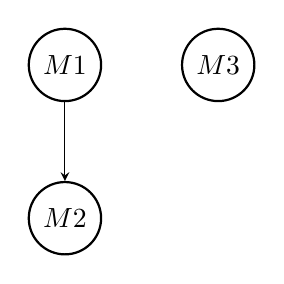
\begin{tikzpicture}[xscale=10, yscale=10,>=stealth]
		\tikzstyle{v}=[circle, minimum size=1mm,draw,thick]
		\node[v] (M1) {$M1$};
		\node[v] (M2) [below=of M1] {$M2$};
		\node[v] (M3) [right=of M1] {$M3$};
		\draw [->] (M1) to (M2);
		\end{tikzpicture}
	\end{center}
	\caption{Grafo de subsunci\'on basado en la Figura~\ref{figures.examples.subsumptionTable}}
	\label{figures.examples.subsumptionGraph}
\end{figure}

\subsection{Acoplamiento}

\emph{Coupling} se define como el acoplamiento entre fallas reales y mutantes, y es una propiedad altamente deseable. Sin la misma, mutation testing perder\'ia su utilidad, ya que no existir\'ia una correlaci\'on entre un mutation score alto y una buena capacidad de parte de la test suite para detectar fallas reales. El trabajo m\'as importante sobre este tema, y uno que nos representa una motivaci\'on importante para el desarrollo de nuestro operador de mutaci\'on presentado en esta tesis, es \cite{bibliography.mutation.evaluation.valid-substitute}. El acoplamiento entre mutantes y fallas reales es una relaci\'on que indica que existe una correlaci\'on positiva entre la capacidad de un conjunto de tests de detectar un conjunto de mutantes, y la capacidad del conjunto de tests en detectar ciertas fallas reales. Por otra parte, el acoplamiento entre diferentes mutaciones (diferentes fallas artificiales) representa una situaci\'on indeseable, similar al caso de equivalencia entre mutantes. Una manera de medir acoplamiento entre un programa, con una falla real conocida, y un conjunto de mutantes, es evaluar si los tests que detectan la falla, son los mismos que detectan al conjunto de mutantes. En el trabajo previamente citado se utiliza esta m\'etrica, aunque con la exigencia adicional de que s\'olo se muta el c\'odigo asociado a la reparaci\'on de la falla real.

%\section{High order}
%
%\texttt{High Order}, la combinaci\'on de mutaciones, generada al aplicar operadores de mutaci\'on m\'as de una vez al generar un mutante, se denominan mutaciones de alto order mientras que aquellas que la forman, se las llama de primer orden. Si bien en principio esto agregar\'ia una gran cantidad de nuevos mutantes\footnote{Usualmente la cantidad de mutantes al aplicar m\'as de una mutaci\'on por mutante est\'a acotada por M$_0^G$ en donde \texttt{M$_0$} son la cantidad de mutantes de primer orden y \texttt{G} son la cantidad de mutaciones por mutante}, los estudios actuales que se enfocan en esta t\'ecnica concluyen que estos mutantes de alto orden representan fallas artificiales m\'as sutiles y que subsumen a una gran cantidad de mutantes de primer orden. [AGREGAR]
